\documentclass[conference]{IEEEtran}

\usepackage{graphicx}
\usepackage{booktabs}
\usepackage{tabularx}
\usepackage{array}
\usepackage{xcolor}
\usepackage{tikz}
\usetikzlibrary{positioning,arrows.meta,calc}
\usepackage{balance}
\usepackage[hidelinks]{hyperref}
\hypersetup{pdftitle={A Reference-Free Summary Evaluation System},pdfauthor={Chen Jinhua}}

\definecolor{navy}{HTML}{172033}
\definecolor{blue}{HTML}{2563EB}
\definecolor{bluefill}{HTML}{E8F0FE}
\definecolor{green}{HTML}{15803D}
\definecolor{greenfill}{HTML}{E9F6EC}
\definecolor{orange}{HTML}{D97706}
\definecolor{purple}{HTML}{7B61A8}
\definecolor{red}{HTML}{B91C1C}
\definecolor{gray}{HTML}{5A6C7D}

\newcolumntype{Y}{>{\raggedright\arraybackslash}X}
\newcolumntype{R}{>{\raggedleft\arraybackslash}p{12mm}}
\newcolumntype{P}[1]{>{\raggedright\arraybackslash}p{#1}}
\renewcommand{\arraystretch}{1.06}
\setlength{\tabcolsep}{4pt}

\tikzset{
  box/.style={rounded corners=1.5pt,draw=navy,very thin,fill=white,align=center,minimum height=7mm,inner xsep=2.4mm,inner ysep=1.5mm,font=\sffamily\scriptsize\bfseries},
  code/.style={box,draw=blue,fill=bluefill},
  agent/.style={box,draw=purple,fill=purple!7},
  semantic/.style={box,draw=orange,fill=orange!8},
  output/.style={box,draw=green,fill=greenfill},
  terminal/.style={box,draw=red,fill=red!6,text=red},
  arrow/.style={-{Stealth[length=1.7mm]},draw=gray,semithick},
  pass/.style={-{Stealth[length=1.7mm]},draw=green,semithick},
  review/.style={-{Stealth[length=1.7mm]},draw=blue,semithick},
  stop/.style={-{Stealth[length=1.7mm]},draw=red,semithick},
  tinylabel/.style={font=\sffamily\fontsize{5.5}{6.2}\selectfont,text=gray,align=center}
}

\title{A Reference-Free Summary Evaluation System\\
\large Two Independently Implemented Plugins for Auditable Japanese News Evaluation}

\author{\IEEEauthorblockN{Chen Jinhua}
\IEEEauthorblockA{AI Quality Scientist Take-Home Assignment\\50 articles, 250 candidate summaries}}

\begin{document}
\maketitle

\begin{abstract}
This work presents a reference-free evaluator for Japanese news summaries. The central design is a funnel: deterministic checks first identify physically verifiable contract violations; assigned-article embedding supplies mandatory relevance evidence; isolated language-model Agents then judge semantic eligibility and graded quality; and an independent Reviewer verifies every terminal decision and score. The evaluator is delivered as an executable Plugin rather than a collection of prompts. A Claude Code Plugin is the primary implementation and produces the submitted scores; a separately implemented Codex Plugin reproduces the same evaluation contract as cross-host validation. Both processed all 250 article--summary pairs. The primary run achieved 91.49\% agreement with offline weak labels and zero planted-bad ranking inversions across 50 articles. The two implementations agreed on routing for 94.4\% of candidates and achieved 0.8907 Spearman correlation on jointly scored candidates. These results support both the evaluation logic and its reproducibility without using reference summaries at runtime.
\end{abstract}

\begin{IEEEkeywords}
LLM evaluation, summary quality, reference-free evaluation, agentic workflow, reproducibility
\end{IEEEkeywords}

\section{Exploration}
\subsection{Dataset and observed populations}
The dataset contains five opaque candidates for each of 50 Japanese XL-Sum articles. Candidate lengths range from 22 to 302 characters (median 125). Manual inspection and targeted probes exposed reference-quality summaries, fluent paraphrases, low-coverage outputs, changed entities and numbers, continuous source copies, unrelated text, incomplete fragments, central factual reversals, and central fabrications. A single similarity score cannot represent these populations faithfully: source copying is highly similar to the article, while on-topic reversals preserve topic vocabulary despite being semantically invalid.

\begin{table}[t]
\caption{Exploration findings translated into design decisions.}
\label{tab:exploration}
\centering
\footnotesize
\begin{tabularx}{\columnwidth}{@{}p{19mm}YY@{}}
\toprule
\textbf{Finding} & \textbf{Rejected shortcut} & \textbf{Decision} \\
\midrule
No runtime human reference & Score against \texttt{reference\_summary} & Restrict runtime evidence to article and candidate. \\
Copies resemble the article & Similarity as quality & Detect copying before semantic scoring. \\
Reversals remain on topic & Embedding as factuality & Use Agents for source-grounded semantics. \\
Peripheral errors remain rankable & Every factual error is terminal & Separate central invalidity from soft penalties. \\
Headline endings resemble cuts & Punctuation-only truncation & Terminate only an unusable fragment. \\
\bottomrule
\end{tabularx}
\end{table}

\subsection{Embedding calibration and anchor ablation}
Two disjoint 10-article experiments tested \texttt{qwen3-embedding:0.6b}. Relevant pairs averaged 0.800 and 0.780; unrelated pairs averaged 0.275 and 0.263. Relevant values were 0.707--0.868 and unrelated values 0.163--0.398, so 0.50 separated all 40 probe pairs. This justified embedding as a required relevance signal, not as an autonomous verdict.

Candidate-to-anchor embedding was tested for coverage. Its small-sample Spearman correlation was higher than article similarity (0.6303 vs. 0.5282), but leave-one-out error was worse (MAE 4.0123 vs. 3.6246; combined features 4.4121). I therefore retained the structured anchor for coverage reasoning without adding a second numerical similarity feature.

\section{Design}
\subsection{Evidence boundary}
The production evaluator never sees a human reference or another article. References join only after both runs are final, exclusively for offline validation. This prevents an evaluation shortcut that would not exist in the real application.

\begin{figure}[t]
\centering
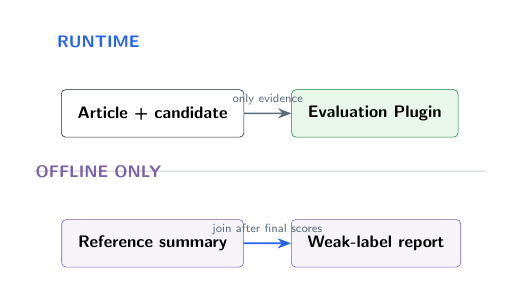
\begin{tikzpicture}[node distance=5mm and 7mm,transform shape,scale=.86]
  \node[font=\sffamily\scriptsize\bfseries,text=blue,anchor=west] (runtime) {RUNTIME};
  \node[box,below=of runtime,xshift=8mm] (input) {Article + candidate};
  \node[output,right=of input] (plugin) {Evaluation Plugin};
  \draw[arrow] (input) -- node[tinylabel,above]{only evidence} (plugin);
  \draw[gray!35,line width=.4pt] ($(input.south west)+(-4mm,-5mm)$) -- ($(plugin.south east)+(4mm,-5mm)$);
  \node[font=\sffamily\scriptsize\bfseries,text=purple,anchor=west,below=15mm of runtime] (offline) {OFFLINE ONLY};
  \node[agent,below=of offline,xshift=8mm] (reference) {Reference summary};
  \node[agent,right=of reference] (weak) {Weak-label report};
  \draw[review] (reference) -- node[tinylabel,above]{join after final scores} (weak);
\end{tikzpicture}
\caption{Runtime and offline evidence are deliberately separated.}
\label{fig:evidence}
\end{figure}

\subsection{Evaluation funnel}
The architecture follows four invariants: code measures and proposes while Agents judge; eligibility precedes graded quality; every consequential decision is reviewed independently; and every output retains a machine-auditable trace.

\begin{figure*}[t]
\centering
\resizebox{0.98\textwidth}{!}{%
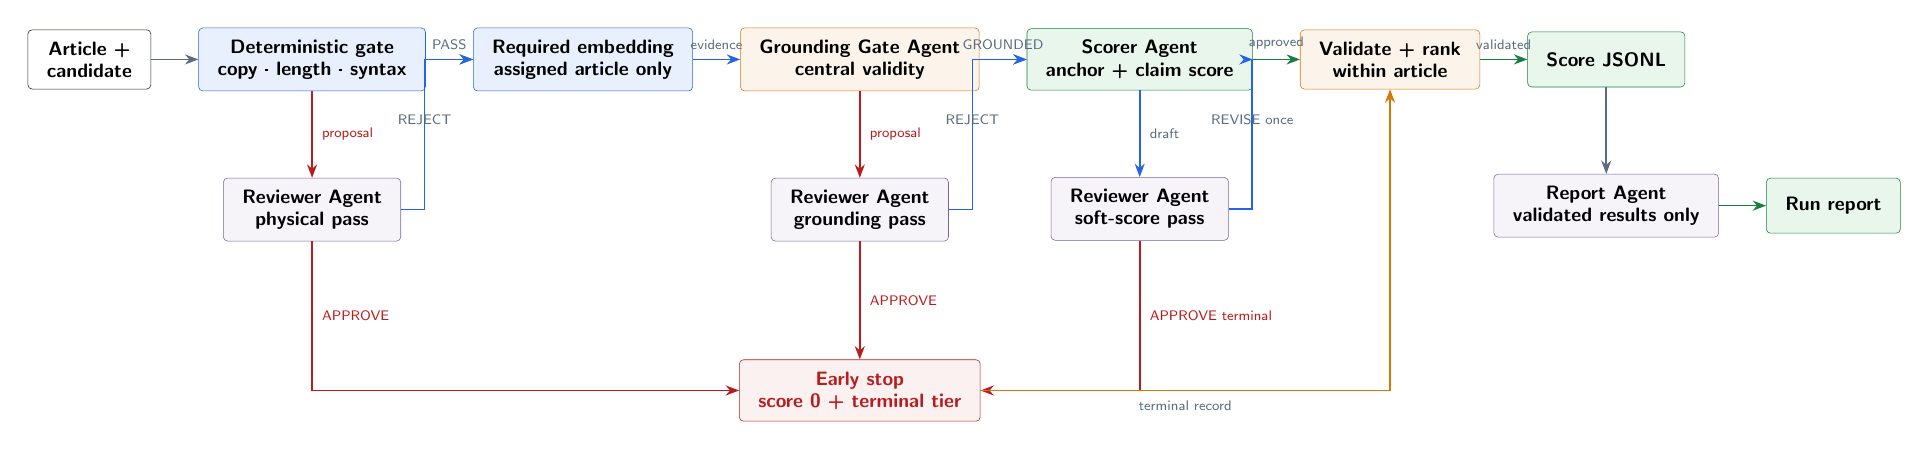
\begin{tikzpicture}[node distance=8mm and 6mm]
  \node[box] (input) {Article +\\candidate};
  \node[code,right=of input] (physical) {Deterministic gate\\copy · length · syntax};
  \node[code,right=of physical] (embedding) {Required embedding\\assigned article only};
  \node[semantic,right=of embedding] (grounding) {Grounding Gate Agent\\central validity};
  \node[output,right=of grounding] (scorer) {Scorer Agent\\anchor + claim score};
  \node[semantic,right=of scorer] (validate) {Validate + rank\\within article};
  \node[output,right=of validate] (jsonl) {Score JSONL};
  \draw[arrow] (input) -- (physical);
  \draw[pass] (physical) -- node[tinylabel,above]{PASS} (embedding);
  \draw[review] (embedding) -- node[tinylabel,above]{evidence} (grounding);
  \draw[pass] (grounding) -- node[tinylabel,above]{GROUNDED} (scorer);
  \draw[pass] (scorer) -- node[tinylabel,above]{approved} (validate);
  \draw[pass] (validate) -- node[tinylabel,above]{validated} (jsonl);
  \node[agent,below=11mm of physical] (physicalreview) {Reviewer Agent\\physical pass};
  \node[agent,below=11mm of grounding] (groundreview) {Reviewer Agent\\grounding pass};
  \node[agent,below=11mm of scorer] (scorereview) {Reviewer Agent\\soft-score pass};
  \node[terminal,below=15mm of groundreview] (terminal) {Early stop\\score 0 + terminal tier};
  \draw[stop] (physical) -- node[tinylabel,right,text=red]{proposal} (physicalreview);
  \draw[stop] (grounding) -- node[tinylabel,right,text=red]{proposal} (groundreview);
  \draw[review] (scorer) -- node[tinylabel,right]{draft} (scorereview);
  \draw[stop] (physicalreview.south) |- node[tinylabel,near start,right,text=red]{APPROVE} (terminal.west);
  \draw[stop] (groundreview) -- node[tinylabel,right,text=red]{APPROVE} (terminal);
  \draw[stop] (scorereview.south) |- node[tinylabel,near start,right,text=red]{APPROVE terminal} (terminal.east);
  \draw[review] (physicalreview.east) -- ++(3mm,0) |- node[tinylabel,near start,above]{REJECT} (embedding.west);
  \draw[review] (groundreview.east) -- ++(3mm,0) |- node[tinylabel,near start,above]{REJECT} (scorer.west);
  \draw[review] (scorereview.east) -- ++(3mm,0) |- node[tinylabel,near start,above]{REVISE once} (scorer.east);
  \node[agent,below=11mm of jsonl] (reporter) {Report Agent\\validated results only};
  \node[output,right=of reporter] (report) {Run report};
  \draw[arrow] (jsonl) -- (reporter);
  \draw[pass] (reporter) -- (report);
  \draw[orange,semithick,-{Stealth[length=1.7mm]}] (terminal.east) -| node[tinylabel,near start,below]{terminal record} (validate.south);
\end{tikzpicture}}
\caption{Complete evaluation funnel. Each Agent role is isolated. Terminal proposals require Reviewer approval; rejection continues to the next eligible stage, while a score revision is bounded to one pass.}
\label{fig:funnel}
\end{figure*}

\subsection{Physical and semantic eligibility}
The deterministic gate normalizes Unicode and whitespace, counts top-level sentences outside paired delimiters, and records copy, length, and truncation evidence. Copying is proposed when the candidate is fully contained in the article for at least 30 normalized characters, or when an exact span of at least 60 characters has at least 0.90 candidate coverage and 0.95 12-character-shingle coverage. More than three sentences violates the product contract. These checks propose terminal outcomes; the physical Reviewer confirms or rejects them.

Every survivor is embedded against the assigned title plus the first 1,500 article characters. One article vector is cached across its five candidates. The trace records similarity, threshold, suspect state, and zero cross-article comparisons. The Grounding Gate Agent then judges only central semantic validity. It may propose \texttt{OFF\_TOPIC}, \texttt{FACTUAL\_REVERSAL}, or \texttt{FABRICATED\_CONTENT}, citing article and candidate spans. A Grounding Reviewer must confirm centrality before score 0 is allowed.

\subsection{Graded quality and independent review}
The Scorer first generates one article-only anchor---main event, key facts, and a short anchor summary---before seeing candidates. It decomposes each candidate into atomic claims and marks each \texttt{SUPPORTED}, \texttt{CONTRADICTED}, or \texttt{NOT\_IN\_SOURCE} with source evidence. Four dimensions sum exactly to 100: faithfulness 50, coverage 30, coherence 15, and conciseness 5. Weighting makes factual reliability dominant while preserving useful differentiation among eligible summaries.

A fresh Reviewer rechecks claim evidence, dimensions, arithmetic, label bands, and trace events. It may approve, request one bounded revision, or confirm a terminal failure missed upstream; scores are never averaged between Agents. Each Agent receives exactly one condition-matched synthetic few-shot, including a peripheral-defect counterexample that discourages over-termination.

\begin{table*}[t]
\caption{Complete output label taxonomy. Terminal labels receive score 0 but retain a separate tier for within-article ordering.}
\label{tab:labels}
\centering
\footnotesize
\begin{tabularx}{0.96\textwidth}{@{}p{43mm}Y@{}}
\toprule
\textbf{Label} & \textbf{Explanation} \\
\midrule
\texttt{EXCELLENT} & Faithful, comprehensive, coherent, and concise; score 90--100. \\
\texttt{GOOD} & Strong and reliable with limited omissions or presentation weaknesses; score 75--89. \\
\texttt{FINE} & Usable and communicates the main event, with one clear gap; score 65--74. \\
\texttt{MIXED} & Partially useful with material factual, coverage, or readability weakness; score 50--64. \\
\texttt{POOR} & Eligible but substantially weak; remains usable enough to compare; score 0--49. \\
\texttt{HARD\_FAIL\_EMPTY} & No usable output. \\
\texttt{HARD\_FAIL\_OFF\_TOPIC} & Unrelated to the assigned article. \\
\texttt{HARD\_FAIL\_REVERSAL} & Reverses the central event, outcome, state, or decision. \\
\texttt{HARD\_FAIL\_FABRICATION} & Central event, quotation, outcome, or load-bearing fact is unsupported. \\
\texttt{HARD\_FAIL\_COPY} & Continuous or near-complete source copy rather than a summary. \\
\texttt{HARD\_FAIL\_TRUNCATION} & Unusable fragment that stops before a complete proposition. \\
\texttt{HARD\_FAIL\_OVER\_LENGTH} & Exceeds the maximum of three sentences. \\
\bottomrule
\end{tabularx}
\end{table*}

Eligible summaries always rank above terminal outputs. Within the terminal set, unrelated, centrally false, fabricated, and empty outputs use tier 0; source copies tier 1; unusable truncations tier 2; and over-length outputs tier 3. The distinction preserves the task's need to order five candidates even when multiple candidates receive score 0.

\subsection{Plugin as executable specification}
The evaluator is delivered as a Plugin: one command activates the evaluation skill, deterministic scripts, isolated Agent roles, rubric, schemas, validators, and deterministic report generation. The Claude Code Plugin is primary and produced \texttt{scores.jsonl}. The Codex Plugin independently implements the same contract using genuine Codex subagents and extra hand-off validators. Only embedding runs locally; local generative models are prohibited for grounding, anchoring, scoring, review, revision, and report conclusions.

\begin{figure}[t]
\centering
\resizebox{0.94\columnwidth}{!}{%
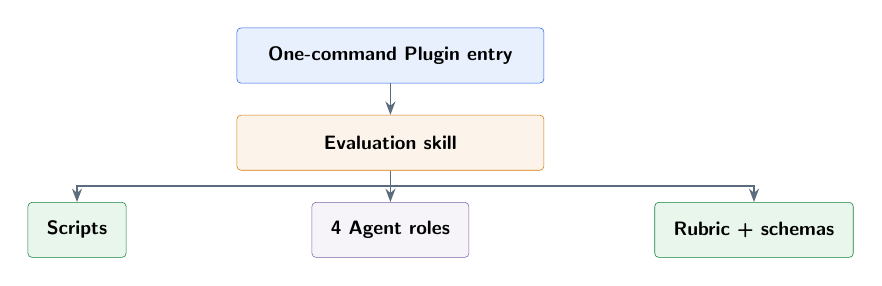
\begin{tikzpicture}[node distance=4mm and 5mm]
  \node[code,minimum width=39mm] (command) {One-command Plugin entry};
  \node[semantic,below=of command,minimum width=39mm] (skill) {Evaluation skill};
  \node[output,below left=of skill,xshift=-9mm] (scripts) {Scripts};
  \node[agent,below=of skill] (agents) {4 Agent roles};
  \node[output,below right=of skill,xshift=9mm] (schema) {Rubric + schemas};
  \draw[arrow] (command) -- (skill);
  \draw[arrow] (skill.south) -- ++(0,-2mm) -| (scripts.north);
  \draw[arrow] (skill) -- (agents);
  \draw[arrow] (skill.south) -- ++(0,-2mm) -| (schema.north);
\end{tikzpicture}}
\caption{The Plugin makes the evaluation design directly executable.}
\label{fig:plugin}
\end{figure}

\section{Validation}
\subsection{Complete independent runs}
Both Plugins evaluated all 250 article--candidate pairs. All output rows passed deterministic schema, arithmetic, ordering, label-band, and trace validators. Table~\ref{tab:runresults} reports every final outcome; Fig.~\ref{fig:distributions} shows the corresponding routing and soft-label distributions.

\begin{table*}[t]
\caption{Complete-run outcomes for both independently orchestrated implementations.}
\label{tab:runresults}
\centering
\footnotesize
\begin{tabular}{@{}lrr@{\qquad}lrr@{}}
\toprule
\textbf{Run metric} & \textbf{Claude} & \textbf{Codex} & \textbf{Final category} & \textbf{Claude} & \textbf{Codex} \\
\midrule
Articles / candidates / valid rows & 50 / 250 / 250 & 50 / 250 / 250 & Verbatim source copy & 50 & 50 \\
Soft-scored candidates & 165 (66.0\%) & 173 (69.2\%) & Off-topic & 16 & 17 \\
Terminal candidates & 85 (34.0\%) & 77 (30.8\%) & Central factual reversal & 13 & 7 \\
Eligible mean / median & 76.07 / 79 & 76.15 / 82 & Obvious truncation & 5 & 3 \\
Eligible range & 35--98 & 28--100 & Central fabrication & 1 & 0 \\
& & & Over length / empty & 0 & 0 \\
\cmidrule(lr){4-6}
& & & \textbf{Terminal total} & \textbf{85} & \textbf{77} \\
\bottomrule
\end{tabular}
\end{table*}

\begin{figure*}[t]
\centering
\begin{minipage}[t]{0.235\textwidth}
  \centering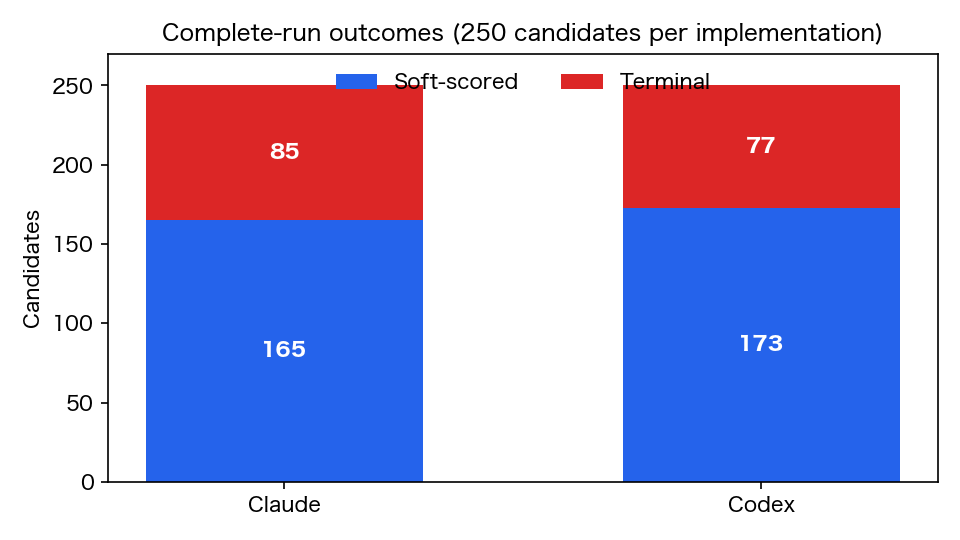
\includegraphics[width=\linewidth]{validation/pipeline_outcomes_comparison.png}\\[-1mm]
  \footnotesize (a) Eligibility routing
\end{minipage}\hfill
\begin{minipage}[t]{0.235\textwidth}
  \centering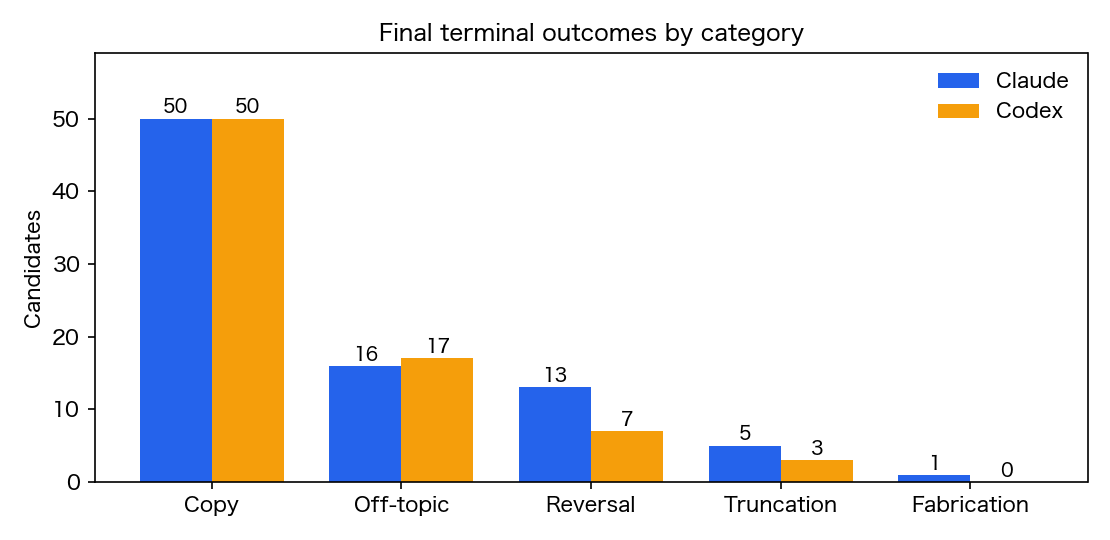
\includegraphics[width=\linewidth]{validation/terminal_category_comparison.png}\\[-1mm]
  \footnotesize (b) Terminal categories
\end{minipage}\hfill
\begin{minipage}[t]{0.235\textwidth}
  \centering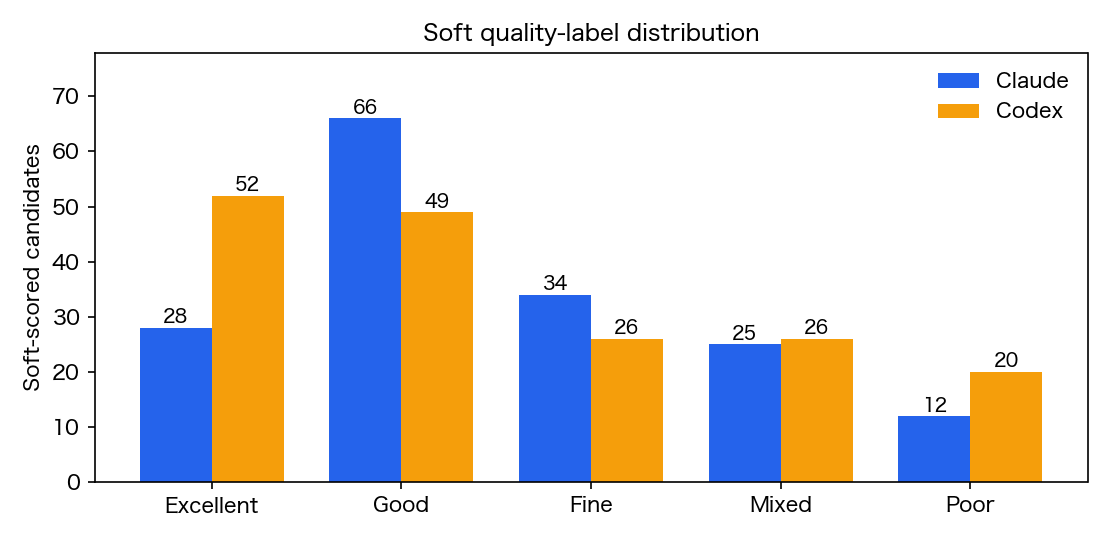
\includegraphics[width=\linewidth]{validation/soft_label_comparison.png}\\[-1mm]
  \footnotesize (c) Eligible quality labels
\end{minipage}\hfill
\begin{minipage}[t]{0.235\textwidth}
  \centering
\includegraphics[width=\linewidth]{validation/score_agreement.png}\\[-1mm]
  \footnotesize (d) Joint-score agreement
\end{minipage}
\caption{Full-dataset validation. The implementations reproduce the same broad routing behavior and strongly preserve eligible-score ordering.}
\label{fig:distributions}
\end{figure*}

\subsection{Offline weak-label validation}
References were withheld during scoring and joined only after both runs were final. This avoids using them as unavailable runtime ground truth while still exploiting their diagnostic value. Both systems retained all 58 reference reproductions; both terminated all 50 source copies and all 16 planted off-topic candidates. On 141 gradable records, the primary Claude run agreed with the offline weak labels on 129 (91.49\%), and Codex agreed on 127 (90.07\%). Most importantly for the five-way ranking task, neither implementation placed a planted-bad candidate above the intended survivor in any of the 50 articles.

\begin{table}[t]
\caption{Offline validation after final scoring.}
\label{tab:offline}
\centering
\footnotesize
\begin{tabularx}{\columnwidth}{@{}Yrr@{}}
\toprule
\textbf{Check} & \textbf{Claude} & \textbf{Codex} \\
\midrule
Reference reproductions survived & 58/58 & 58/58 \\
Source copies terminated & 50/50 & 50/50 \\
Off-topic candidates terminated & 16/16 & 16/16 \\
Weak-label agreement & 129/141 & 127/141 \\
& 91.49\% & 90.07\% \\
Planted-bad inversions & \textbf{0/50} & \textbf{0/50} \\
\bottomrule
\end{tabularx}
\end{table}

\subsection{Cross-host replication}
The independent implementations provide a stronger test than rerunning one prompt. They agree on terminal versus graded routing for 236/250 candidates (94.4\%). Among the 74 candidates both route to terminal, the terminal category agrees on all 74. For the 162 candidates both grade, score ordering has Spearman correlation 0.8907 and mean absolute difference 6.85 points. The joint-set means are also close: 76.27 for Claude and 78.23 for Codex. Thus, different Agent hosts reproduce both the funnel's routing and the relative ordering of eligible candidates.

\begin{table}[t]
\caption{Agreement between independent Plugin implementations.}
\label{tab:cross}
\centering
\footnotesize
\begin{tabularx}{\columnwidth}{@{}YR@{}}
\toprule
\textbf{Measure} & \textbf{Result} \\
\midrule
Both terminal / both graded & 74 / 162 \\
Claude-only / Codex-only terminal & 11 / 3 \\
Routing agreement & \textbf{236/250 (94.4\%)} \\
Shared terminal-category agreement & \textbf{74/74 (100\%)} \\
Joint-score Spearman & \textbf{0.8907} \\
Mean absolute score difference & 6.85 \\
Joint mean, Claude / Codex & 76.27 / 78.23 \\
\bottomrule
\end{tabularx}
\end{table}

\begin{table*}[t]
\caption{Validation argument: each central design claim is supported by an independent observable result.}
\label{tab:argument}
\centering
\footnotesize
\begin{tabularx}{0.96\textwidth}{@{}P{30mm}@{\hspace{3mm}}P{38mm}@{\hspace{3mm}}P{34mm}@{\hspace{3mm}}Y@{}}
\toprule
\textbf{Claim} & \textbf{Validation test} & \textbf{Observed result} & \textbf{Interpretation} \\
\midrule
The funnel identifies outputs that are not usable summaries & Planted source-copy and off-topic populations & Both Plugins: 50/50 copies and 16/16 off-topic candidates terminated & The clearest eligibility failures are detected consistently without a runtime reference. \\
The evaluator does not reject strong summaries indiscriminately & Offline join against 58 reference reproductions & Both Plugins: 58/58 survived & Terminal gates preserve a known high-quality population. \\
The final ordering is safe for the five-candidate task & Compare the planted-bad candidate with intended survivors within every article & Both Plugins: 0/50 ranking inversions & Terminal tiers and graded scores place planted failures below useful candidates. \\
The design is reproducible across Agent hosts & Independent Claude and Codex implementations & 94.4\% routing agreement; 0.8907 score Spearman & The result follows the evaluation contract rather than one host-specific prompt trajectory. \\
\bottomrule
\end{tabularx}
\end{table*}

\newpage
\balance
\section{Limitations and Future Work}
The present evidence covers 250 Japanese news summaries. The next experiment should apply the same Plugin-based funnel to larger datasets and to additional languages, testing whether routing, label calibration, and cross-host agreement remain consistent across broader data distributions and multilingual inputs.

\section{Conclusion}
The primary contribution is a reference-free evaluation architecture that separates eligibility from graded quality and assigns each method only the authority its evidence supports. Deterministic checks establish physical facts; embedding supplies mandatory assigned-article relevance evidence; isolated Agents judge central semantic validity and graded quality; independent Reviewers verify every consequential decision; and deterministic validators assemble ranked JSONL and reports. Delivering the design as two installable Plugins makes it executable and reproducible rather than prompt-dependent. The full 250-pair evaluation, 91.49\% primary weak-label agreement, zero planted-bad inversions, 94.4\% cross-host routing agreement, and 0.8907 score correlation jointly support the reliability of the resulting scores.

\end{document}
